% A0: https://de.onlineprinters.ch 86,10 x 120,90 cm with endformat of 84,10 x 118,90 cm
\documentclass[portrait,final,paperwidth=84.10cm, paperheight=118.90cm,showframe fontscale=0.277,margin=1.5cm]{baposter}
\usepackage{relsize}
\usepackage{graphicx}
\usepackage[utf8]{inputenc}
\usepackage[noend]{algorithm}
\usepackage[noend]{algorithmic}
\usepackage{enumitem}
\usepackage[style=ieee, backend=bibtex]{biblatex}
\addbibresource{poster-unsure.bib}
\usepackage{setspace}

% Package list
\usepackage{blindtext}
\usepackage{amsmath,amsthm,amssymb,latexsym} 
\usepackage{times}
\usepackage{xcolor}
\usepackage{hyperref}
\hypersetup{colorlinks,
	citecolor=black,
	filecolor=black,
	linkcolor=black,
	urlcolor=lightgray
}
\sloppy

\usepackage{booktabs} % Top and bottom rules for tables
\usepackage{microtype}

\newcommand{\shrink}{-15pt}
\def\imagetop#1{\vtop{\null\hbox{#1}}}

\RequirePackage{wrapfig}


% Document
\begin{document}
%%%%%%%%%%%%%%%%%%%%%%%%%%%%%%%%%%%%%%%%%%%%%%%%%%%%%%%%%%%%%%%%%%%%%%%%%%%%%%
%%% Here starts the poster
%%%---------------------------------------------------------------------------
%%% Format it to your taste with the options
%%%%%%%%%%%%%%%%%%%%%%%%%%%%%%%%%%%%%%%%%%%%%%%%%%%%%%%%%%%%%%%%%%%%%%%%%%%%%%
% Define some colors
\definecolor{mintish}{RGB}{165,215,210} % Defines the color used for the background
\definecolor{anthrazit}{RGB}{45,55,60}   % Defines the color used for content header

\hyphenation{resolution occlusions}
%%
\begin{poster}%
	% Poster Options
	{
		% Show grid to help with alignment
		grid=false,
		% Column spacing
		colspacing=1.5em,
		columns=4,
		% Color style
		bgColorOne=mintish,
		bgColorTwo=red,
		titleColor=anthrazit,
		footerColor=anthrazit,
%		bgColorTitle=white,
		borderColor=green,
		headerColorOne=anthrazit,
		headerColorTwo=anthrazit,
		headerFontColor=white,
		boxColorOne=white,
		boxColorTwo=white,
		% Format of textbox
		textborder=none,
		% Format of text header
		eyecatcher=false,
		headerborder=none,
		headerheight=0.10\textheight,
		textfont=professionalfonts, %An example of changing the text font
		headershape=rectangle, % rectangle, rounded, smallrounded, roundedleft, roundedright
		headershade=plain, % shade-lr, shade-tb, shade-tb-inverse, plain
		headerfont=\large\bf\textsc, %Sans Serif
		textfont={\setlength{\parindent}{1.5em}},
		boxshade=plain,
		background=plain, % shadeLR, shadeTB, user, none
		titlebackground=plain, % plain, none
		footerbackground=plain, % plain, none
		linewidth=2pt,
		boxpadding=0.8em,
	}
	% Eye Catcher
	{
		
\includegraphics[height=4.0em]{logo/UniBas_Logo_EN_Weiss_Trans_RGB_55}
	} 
	% Title
	{\textcolor{white}{\Huge\bf\textsc{Probabilistic Surface Reconstruction \\with Unknown Correspondence}}\vspace{0.2em}}
	% Authors
	{\textcolor{white}{\normalsize{
				\hspace{-0.2em}\textbf{\underline{Dennis Madsen}}, Thomas Vetter and Marcel Lüthi\\
				Department of Mathematics and Computer Science, University of Basel
			%	\{dennis.madsen, thomas.vetter, marcel.luethi\}@unibas.ch
			}
		}
	}
	% University logo
	{% The makebox allows the title to flow into the logo, this is a hack because of the L shaped logo.
			
\includegraphics[height=6.0em]{logo/UniBas_Logo_EN_Weiss_Trans_RGB_55_UNSURE}
	}
	% Footer
	{
		{\textcolor{lightgray}{\normalsize{\bf{
						\noindent \url{gravis.dmi.unibas.ch}\hfill \url{https://scalismo.org}\hfill \href{mailto:dennis.madsen@unibas.ch}{dennis.madsen@unibas.ch} 
					}
				}
			}
		}
	}
	
	%%%%%%%%%%%%%%%%%%%%%%%%%%%%%%%%%%%%%%%%%%%%%%%%%%%%%%%%%%%%%%%%%%%%%%%%%%%%%%
	%%% Now define the boxes that make up the poster
	%%%---------------------------------------------------------------------------
	%%% Each box has a name and can be placed absolutely or relatively.
	%%% The only inconvenience is that you can only specify a relative position 
	%%% towards an already declared box. So if you have a box attached to the 
	%%% bottom, one to the top and a third one which should be in between, you 
	%%% have to specify the top and bottom boxes before you specify the middle 
	%%% box.
	%%%%%%%%%%%%%%%%%%%%%%%%%%%%%%%%%%%%%%%%%%%%%%%%%%%%%%%%%%%%%%%%%%%%%%%%%%%%%%

	%%%%%%%%%%%%%%%%%%%%%%%%%%%%%%%%%%%%%%%%%%%%%%%%%%%%%%%%%%%%%%%%%%%%%%%%%%%%%%
	\headerbox{Problem}{name=problem,column=0,row=0, span=1}{
	%%%%%%%%%%%%%%%%%%%%%%%%%%%%%%%%%%%%%%%%%%%%%%%%%%%%%%%%%%%%%%%%%%%%%%%%%%%%%%
	\noindent Modelling the posterior distribution of triangulated surface reconstructions from partial data.
	% ESTIMATE the REAL 
}
	
		
	%%%%%%%%%%%%%%%%%%%%%%%%%%%%%%%%%%%%%%%%%%%%%%%%%%%%%%%%%%%%%%%%%%%%%%%%%%%%%%
	\headerbox{Contributions}{name=contribution,column=0,row=0, span=1, below=problem}{
	%%%%%%%%%%%%%%%%%%%%%%%%%%%%%%%%%%%%%%%%%%%%%%%%%%%%%%%%%%%%%%%%%%%%%%%%%%%%%%
	\begin{itemize}[leftmargin=*]
		\item Modelling the posterior distribution of surface reconstructions from a partial surface, without assuming a fixed point-to-point correspondence.
		\item New proposal using geometry information, for faster convergence.
		\item We show the limitations of the analytical posterior.
	\end{itemize}
	\vspace{0.5em}
}
	
	%%%%%%%%%%%%%%%%%%%%%%%%%%%%%%%%%%%%%%%%%%%%%%%%%%%%%%%%%%%%%%%%%%%%%%%%%%%%%%
	\headerbox{Overview}{name=overview,column=1,row=0, span=3, bottomaligned=contribution}{
	%%%%%%%%%%%%%%%%%%%%%%%%%%%%%%%%%%%%%%%%%%%%%%%%%%%%%%%%%%%%%%%%%%%%%%%%%%%%%%
	\begin{center}
	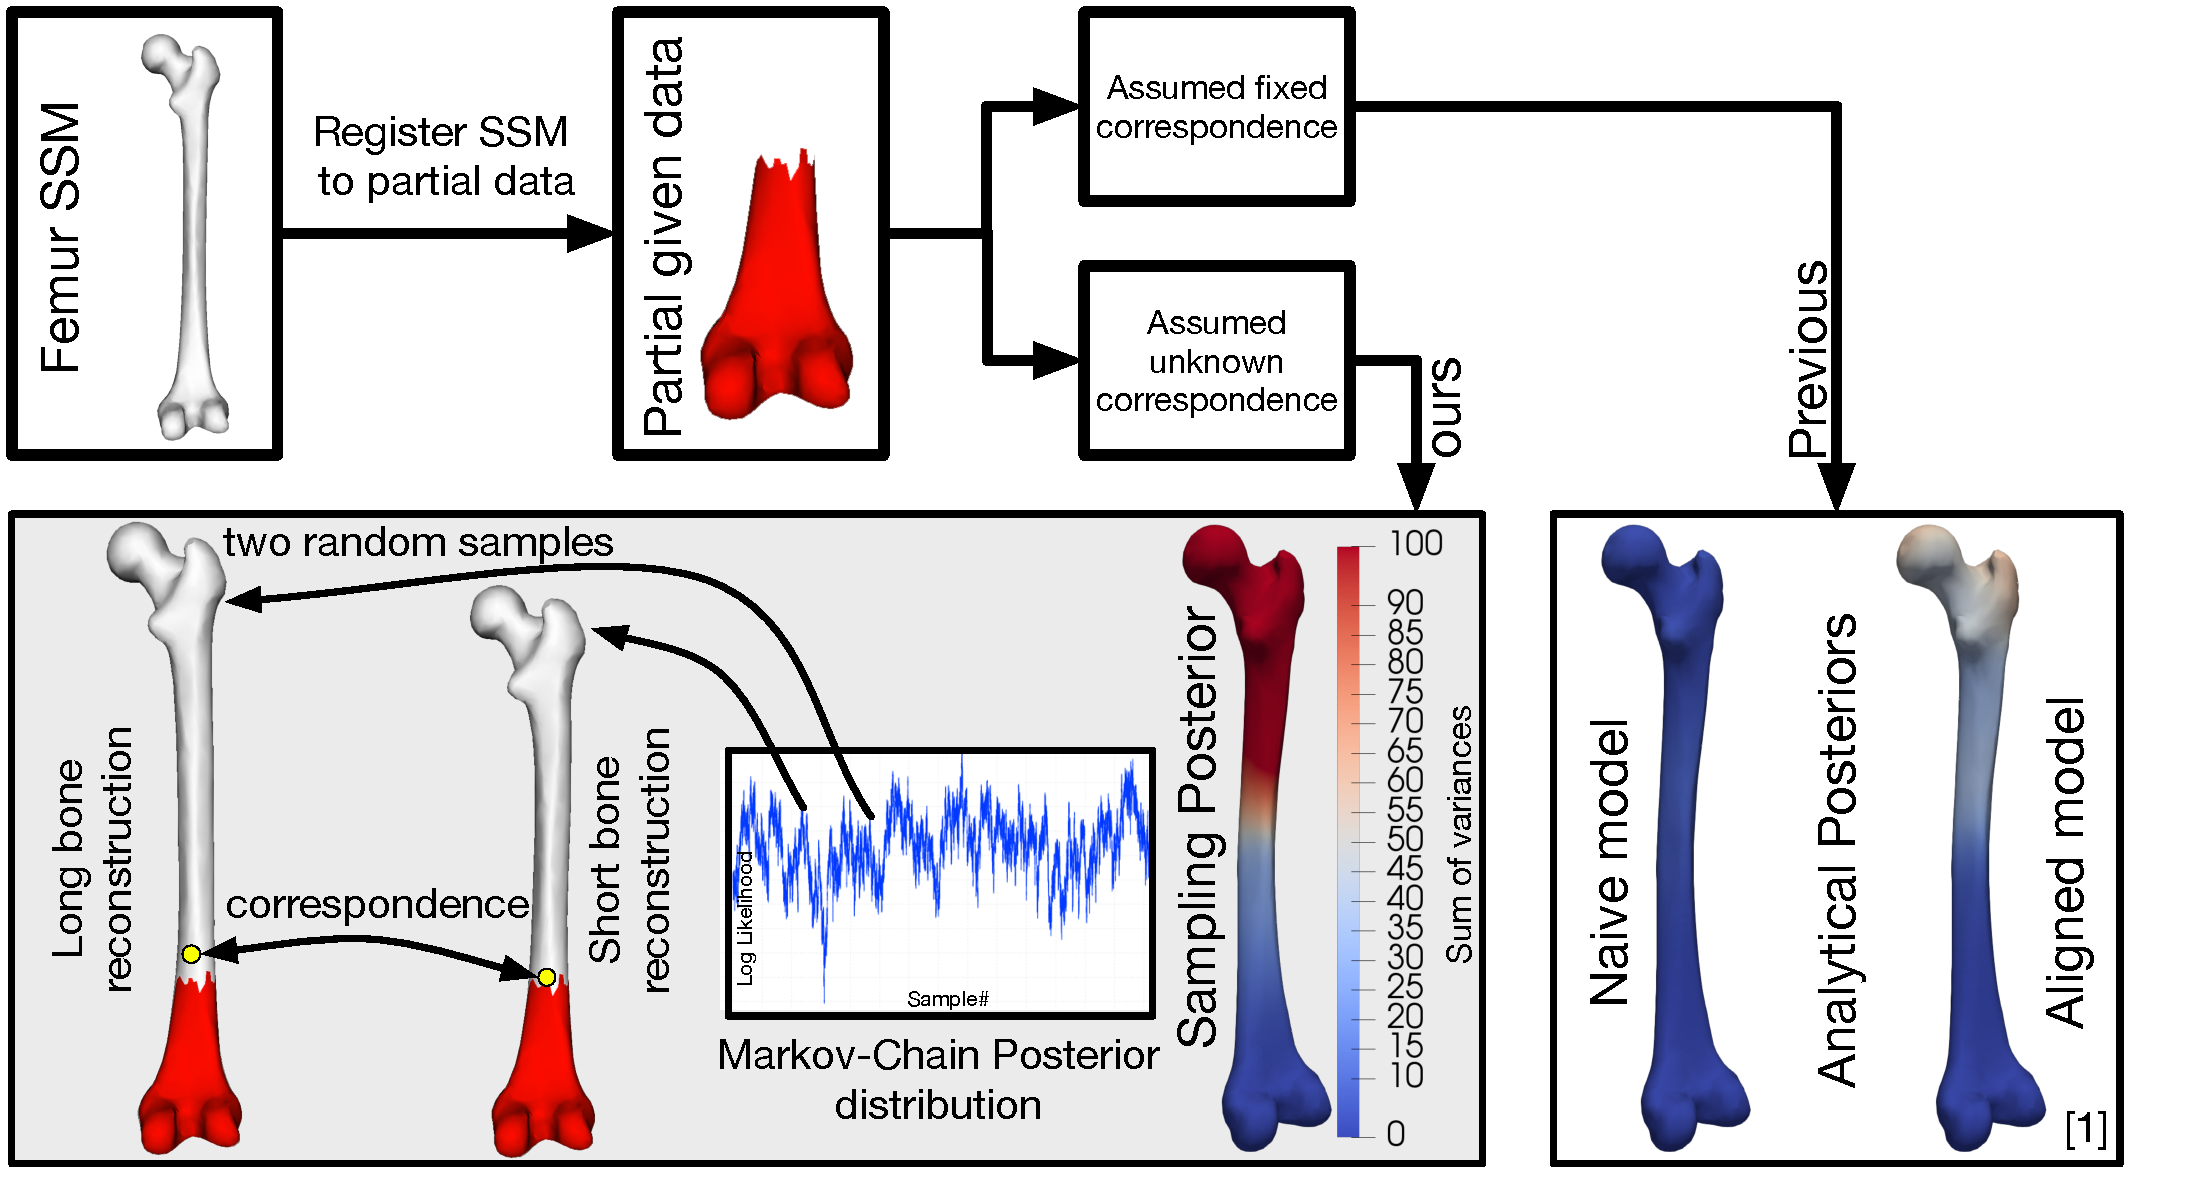
\includegraphics[width=0.9\textwidth]{img/motivation.pdf}
	\end{center}
}
	
	%%%%%%%%%%%%%%%%%%%%%%%%%%%%%%%%%%%%%%%%%%%%%%%%%%%%%%%%%%%%%%%%%%%%%%%%%%%%%%
	\headerbox{Statistical Shape Models}{name=ssm,column=0,row=0, span=2, below=overview}{
	%%%%%%%%%%%%%%%%%%%%%%%%%%%%%%%%%%%%%%%%%%%%%%%%%%%%%%%%%%%%%%%%%%%%%%%%%%%%%%
	\noindent Statistical shape models (SSM) are linear models of shape variation learned from data. PCA leads to a parametric model of the form:
	\[
	\vec{s}= \vec{\mu}+UD\vec{\alpha}= \vec{\mu} + \sum_{i=1}^n \alpha_i \sqrt{\lambda}_i \vec{u}_i, \; \alpha_i \sim \mathcal{N}(0,1)
	\]
	\textbf{The Analytical Posterior Distribution:}\\
	Albrecht et al. showed how to compute the analytical posterior distribution $P(\vec{\alpha}|\vec{s}_{g})$ in \cite{albrecht_posterior_2013} with $\vec{s}_{g}$ being the partial data information modelled with an SSM:
	$\vec{s}_{g}=\vec{\mu}_{g}+U_{g}D_{g}\vec{\alpha}+I_{3q}\epsilon$ and $\epsilon\sim \mathcal{N}(0,\sigma^{2})$
	modelling the noise of the observed partial data.
    \\\\\textbf{Shape and Pose Representation:}
	\begin{itemize}
		\itemsep0.2em 
		\item Translation: $\vec{t}=(t_{x}, t_{y}, t_{z})^{T}\in \mathbb{R}^{3}$.
		\item Rotation: $R(\phi, \psi, \rho)\in SO(3)$
		\item $\vec{\theta}=(\alpha_{0},\ldots,\alpha_{N-1}, \phi, \psi, \rho, t_{x}, t_{y}, t_{z})^{T}$
	\end{itemize}
}

	%%%%%%%%%%%%%%%%%%%%%%%%%%%%%%%%%%%%%%%%%%%%%%%%%%%%%%%%%%%%%%%%%%%%%%%%%%%%%%
	\headerbox{Metropolis-Hastings}{name=mh,column=0, span=2, below=ssm}{
	%%%%%%%%%%%%%%%%%%%%%%%%%%%%%%%%%%%%%%%%%%%%%%%%%%%%%%%%%%%%%%%%%%%%%%%%%%%%%%
	\noindent The \textit{Sampling Posterior} is computed as a Markov-Chain using the Metropolis-Hastings algorithm:
	\begin{center}
		\begin{spacing}{1.2}
		\begin{algorithmic}[1]
			\STATE $\vec{\theta}_0 \leftarrow$ arbitrary initialisation
			\FOR{$i=0$ to S}
			\STATE $\vec{\theta}' \leftarrow$ sample from $Q(\vec{\theta}'|\vec{\theta}_i)$
			\STATE $t \leftarrow  \dfrac{q(\vec{\theta}_i|\vec{\theta}')p(\Gamma_{T}|\vec{\theta}')p(\vec{\theta}')}
			{q(\vec{\theta}'|\vec{\theta}_i)p(\Gamma_{T}|\vec{\theta}_i)p(\vec{\theta}_i)}.$ \COMMENT{acceptance threshold}  \label{algo:sampling:acceptance}
			\STATE $r \leftarrow$ sample from $\mathcal{U}(0,1)$
			\IF{$t > r$}
			\STATE $\vec{\theta}_{i+1} \leftarrow \vec{\theta}'$
			\ELSE
			\STATE $\vec{\theta}_{i+1} \leftarrow \vec{\theta}_{i}$
			\ENDIF
			\ENDFOR
		\end{algorithmic}
	\end{spacing}
	\vspace{-0.2em}
	\end{center}
	}

	%%%%%%%%%%%%%%%%%%%%%%%%%%%%%%%%%%%%%%%%%%%%%%%%%%%%%%%%%%%%%%%%%%%%%%%%%%%%%%
	\headerbox{Results - Correspondence sensitivity}{name=resultsl,column=0,span=2,below=mh, above=bottom}{
	%%%%%%%%%%%%%%%%%%%%%%%%%%%%%%%%%%%%%%%%%%%%%%%%%%%%%%%%%%%%%%%%%%%%%%%%%%%%%%
	\begin{center}
		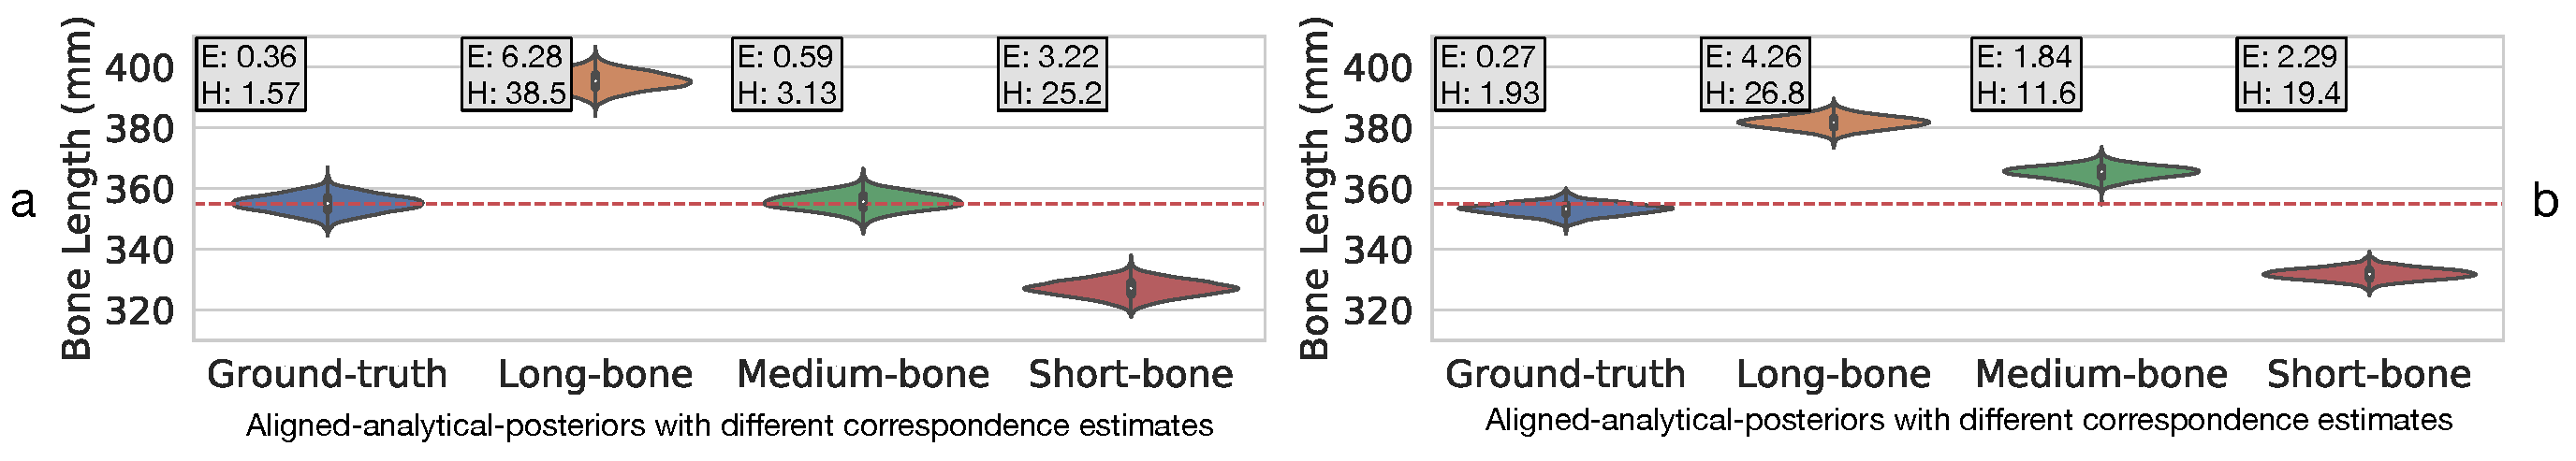
\includegraphics[width=1.0\textwidth]{img/violinPlots_analyticCompare.pdf}
	\end{center}
	
}

	\headerbox{Informed Projection Proposal}{name=proposal,column=2, span=2, below=overview}{
	%%%%%%%%%%%%%%%%%%%%%%%%%%%%%%%%%%%%%%%%%%%%%%%%%%%%%%%%%%%%%%%%%%%%%%%%%%%%%%
	\noindent The standard random-walk proposal $Q$, requires a very small step size to keep the model fixed around the partial data $\vec{s}_{g}$. We introduce the informed projection proposal which keeps the model fixed at the known part of the model $\vec{s_{g*}}$. 
	\begin{enumerate}[leftmargin=*]
		\itemsep0.2em 
		\item Compute corresponding points, $\vec{s_{g*}}$ (\textcolor{red}{red}).
		\item Propose a random pose update $\vec{\theta}_o$ (\textcolor{blue}{blue}), with fixed shape parameters $\vec{\alpha}$.
		\item Compute analytical-posterior $p(\vec{\alpha}|\vec{\theta}_o,\vec{s}_{g*})$ based on $\vec{s}_{g*}$.
		\item Draw a sample shape $\Gamma_p$ (\textcolor{green}{green}) from the posterior distribution (\textcolor{gray}{gray}).
		\item Compute $\vec{\theta}'$ from $\Gamma_p$ on the full SSM $p(\vec{\alpha})$ (\textcolor{green}{green}).
	\end{enumerate}

	\begin{center}
		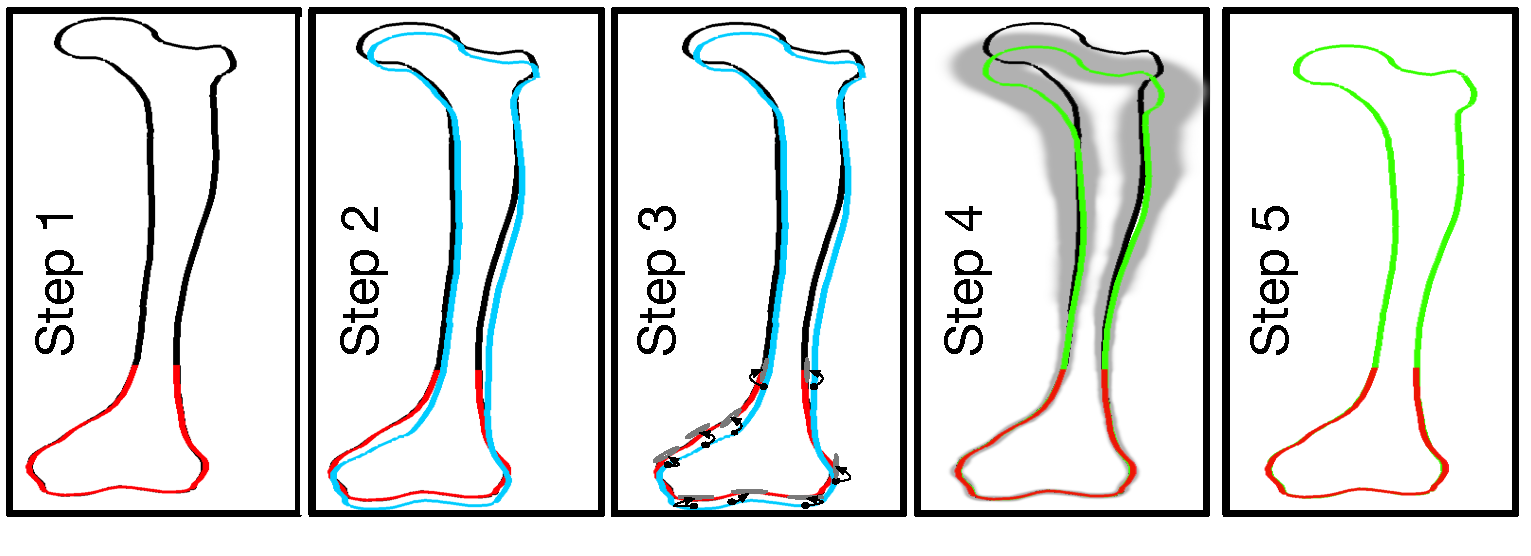
\includegraphics[width=0.9\textwidth]{img/proposal-visualization}
	\end{center}

	\large{\textbf{Transition probability:}}
	\normalsize{
	\begin{itemize}
		\itemsep0em 
		\item $q(\vec{\theta_i}|\vec{\theta}')$ $\rightarrow$ sampling $\vec{\alpha}$ from $p(\vec{\alpha}|\vec{\theta}_o,\vec{s}_{g*})$ (from step 3)
		\item $q(\vec{\theta}'|\vec{\theta_i})$ $\rightarrow$ sampling $\vec{\alpha}'$ from $p(\vec{\alpha}'|\vec{\theta},\vec{s}_{g*})$
	\end{itemize}
}
}


	%%%%%%%%%%%%%%%%%%%%%%%%%%%%%%%%%%%%%%%%%%%%%%%%%%%%%%%%%%%%%%%%%%%%%%%%%%%%%%
	\headerbox{Results - Analytical vs Sampling posterior}{name=resultr,column=2, span=2, below=proposal}{
	%%%%%%%%%%%%%%%%%%%%%%%%%%%%%%%%%%%%%%%%%%%%%%%%%%%%%%%%%%%%%%%%%%%%%%%%%%%%%%
	\begin{center}
		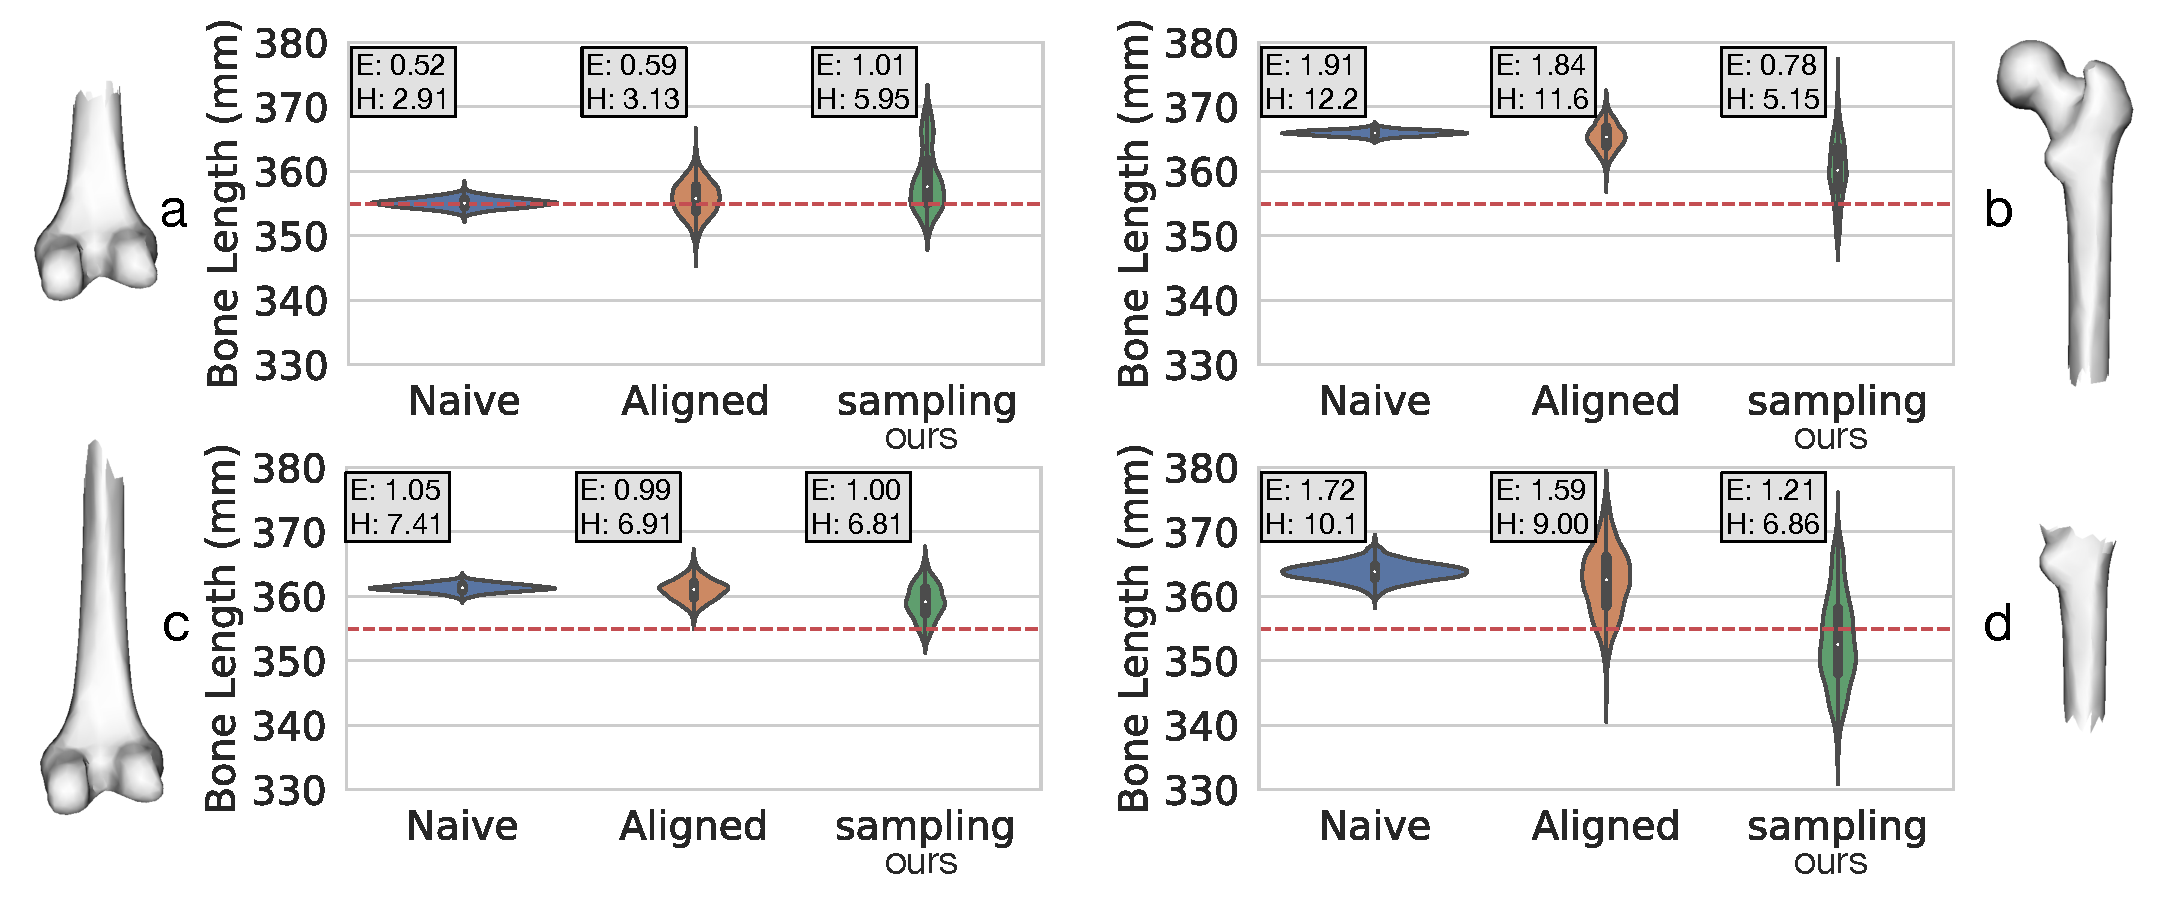
\includegraphics[width=1.0\textwidth]{img/violinPlots_methodCompare.pdf}
	\end{center}
}


	%%%%%%%%%%%%%%%%%%%%%%%%%%%%%%%%%%%%%%%%%%%%%%%%%%%%%%%%%%%%%%%%%%%%%%%%%%%%%%
	\headerbox{References}{name=resultr2,column=2, span=2, below=resultr, above=bottom}{
	%%%%%%%%%%%%%%%%%%%%%%%%%%%%%%%%%%%%%%%%%%%%%%%%%%%%%%%%%%%%%%%%%%%%%%%%%%%%%%
	\AtNextBibliography{\scriptsize}
	\printbibliography[heading=none]
}
\end{poster}

\end{document}